\subsubsection{word2vec} % (fold)
\label{sub:own_word2vec}
As shown in \autoref{fig:w2v-pipeline}, we use the word2vec implementation of the \textit{gensim} library to train language models on both word2vec architectures, with and without pre-processing the requirements through our NLP pipeline before. The outcome are 50-dimensional word vectors which form the basis for our clustering. With our dataset being relatively small, the created vectors may not capture all the semantic regularities, though\,\cite{mikolov_distributed_2013}. We therefore also use the word vectors Mikolov et al. created in order to measure the performance of their word2vec architectures, in 2013\,\cite{mikolov_efficient_2013}. Instead of the approximately 50.000 words in the \crowdre{} dataset, they trained their language model on the Google News dataset with 100 billion words. We thus expect the quality of these word vectors to be much higher and as such to positively affect our later results.
\begin{figure}[ht]
  \begin{center}
    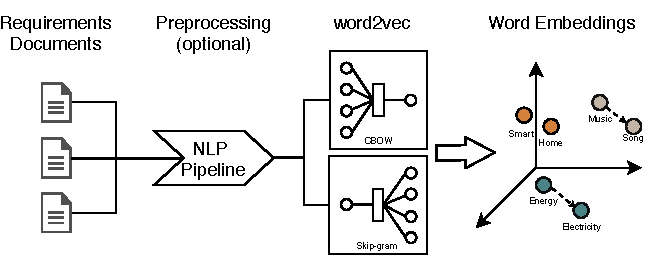
\includegraphics[width=0.9\textwidth]{figures/word2vec_pipeline.pdf}
    \caption{Training a language model on our requirements corpus to create word embeddings using word2vec.}
    \label{fig:w2v-pipeline}
  \end{center}
\end{figure}
\FloatBarrier

With the word embeddings, every word in the \crowdre{} dataset can be represented as a multidimensional vector. We could now create a matrix, representing the whole vocabulary in word vectors, as shown in \autoref{fig:embeddings_matrices} (1). Applying K-Means to the matrix, we would then cluster all the words in the dataset into topics. To cluster the dataset on a sentence level instead, we perform the following four steps:

\begin{enumerate}
\item We create a matrix for every sentence in the corpus, by replacing each word with its vector representation (see \autoref{fig:embeddings_matrices} (2)). The x-dimension of the matrix depends on the length of the sentence, the y-dimension is determined by the length of the word vectors. Using our own 50-dimensional word vectors and e.g. a sentence with 10 words, the shape of the matrix will be $10\times50$.
\item As the sentences in the dataset are of different lengths, the x-dimensions of the matrices are different, too. We use Principal Component Analysis (PCA)\,\cite{wold_principal_1987} to reduce the different x-dimensions to length of the shortest sentence (or the lowest x-dimension respectively).
\item We combine all these sentence matrices in a single matrix $T$, which is a 3-dimensional matrix of the form $T\in\mathbb{R}^{n \times d \times s}$, where $n$ is the total number of sentences, $d$ is the dimension of the word vectors and $s$ is the length of the shortest sentence in the dataset.
\item To cluster our results with K-Means, we need to further transform this matrix into two-dimensional space. We do this by reshaping the matrix $T$ to a matrix $T'$ with $T' \in \mathbb{R}^{n \times d * s}$\footnote{This is done using the reshape-function of the numpy array implementation: \url{https://www.w3resource.com/numpy/manipulation/reshape.php}}.
\end{enumerate}
Finally, we cluster the sentences by applying K-Means to the resulting matrix $T'$.

\begin{figure}[ht]
  \begin{center}
    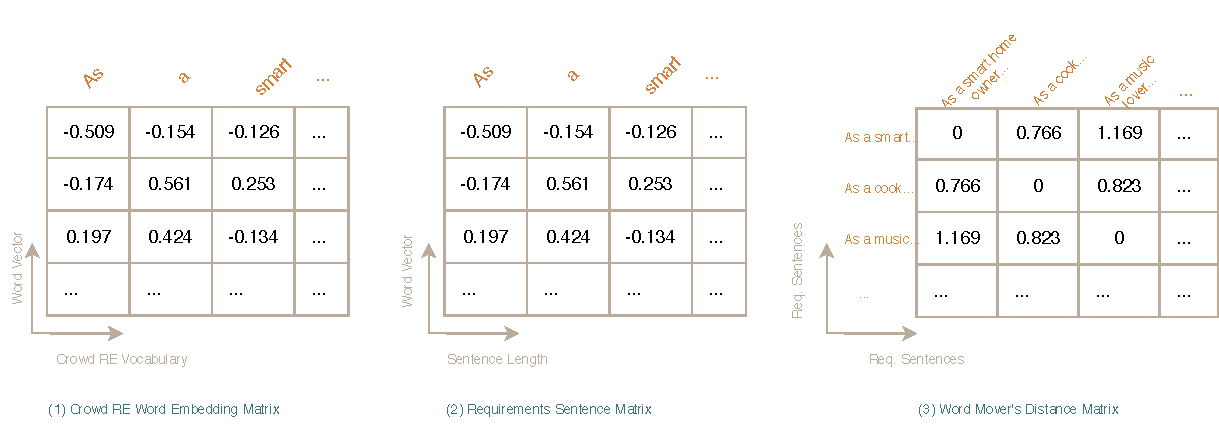
\includegraphics[width=\textwidth]{figures/embedding_matrices.pdf}
    \caption{Representing the \crowdre{} dataset using word embeddings.}
    \label{fig:embeddings_matrices}
  \end{center}
\end{figure}




\begin{figure}[ht]
  \begin{center}
    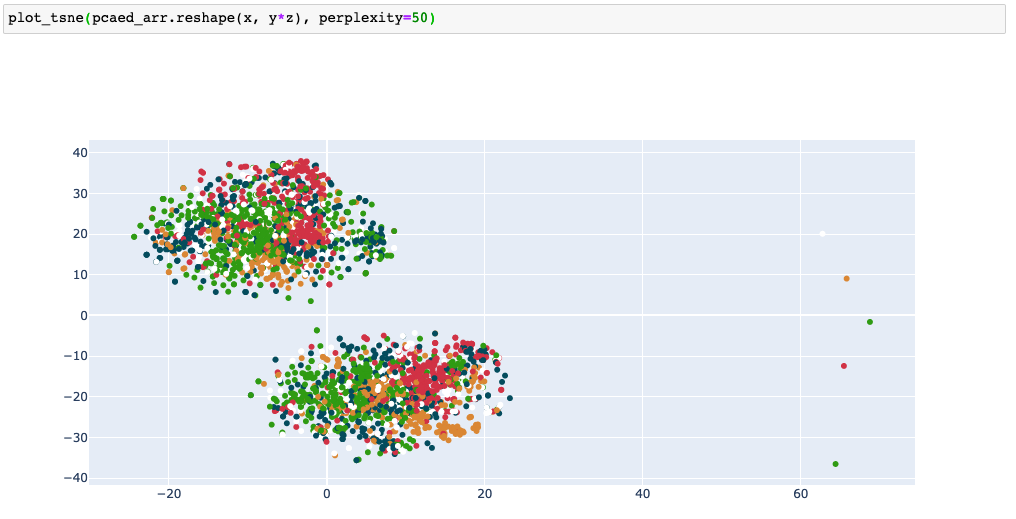
\includegraphics[width=\textwidth]{screenshots/google_word_2_vec_tsne_opti4.png}
    \caption{word2vec result of the clustering with a pretrained model (plotted with t-SNE\,\cite{maaten_visualizing_2008})}
    \label{fig:w2v-pretrained-4}
  \end{center}
\end{figure}
\FloatBarrier